\documentclass[16pt]{article}
\usepackage[russian]{babel}
\usepackage{a4wide}
\usepackage[utf8]{inputenc}
\usepackage{graphicx}
\usepackage{amsmath}
\usepackage{amssymb}
\usepackage{amsthm}
\usepackage{import}
\usepackage{xifthen}
\usepackage{pdfpages}
\usepackage{transparent}
\usepackage{multicol}
\usepackage{animate}
\usepackage{indentfirst}

\newcommand{\incfig}[2]{%
    \def\svgwidth{#2 mm}
    \import{./figures/}{#1.pdf_tex}
}

\newtheorem{Th}{Теорема}
\newtheorem{Lem}{Лемма}
\newenvironment{Proof}{\par\noindent{\bf Доказательство.}}{\hfill$\scriptstyle\blacksquare$}
\newenvironment{Sol}{\par\noindent{\it Решение:}}


\DeclareMathOperator{\Arccos}{arccos}
\DeclareMathOperator{\Arctg}{arctg}
\DeclareMathOperator{\Cl}{Cl}
\DeclareMathOperator{\Ker}{ker}
\DeclareMathOperator{\Ima}{im}
\DeclareMathOperator{\Inter}{int}
\DeclareMathOperator*{\Argmax}{Argmax}
\DeclareMathOperator*{\Var}{var}
\DeclareMathOperator{\Det}{det}
\DeclareMathOperator{\Tr}{tr}
\DeclareMathOperator{\Rea}{re}


\newcommand\Col[2]{\begin{bmatrix}
#1 \\ #2
\end{bmatrix}}
\newcommand\Real{\mathbb{R}} 
\newcommand\A{(\cdot)} 
\newcommand\Sup[2]{\rho( #1 \, | \, #2 )}
\newcommand\Sum[2]{\sum\limits_{#1}^{#2}}
\newcommand\Scal[2]{\langle #1,\, #2 \rangle}
\newcommand\Norm[1]{\left\| #1 \right\|}
\newcommand\Int[2]{\int\limits_{#1}^{#2}}
\newcommand\PS{\mathcal{P}}
\newcommand\X{\mathcal{X}} 
\newcommand\Pict[3]{
\begin{figure}[h!]
    \centering
    \incfig{#1}{#3}
    \caption{#2}
    \label{fig:#1}
\end{figure}
}


\begin{document}

\thispagestyle{empty}

\begin{center}
\ \vspace{-3cm}


\includegraphics[width=0.5\textwidth]{msu.eps}\\
{\scshape Московский государственный университет имени М.~В.~Ломоносова}\\
Факультет вычислительной математики и кибернетики\\
Кафедра системного анализа

\vfill

{\LARGE Отчёт по заданию 2 курсовой работы}

\vspace{1cm}

{\Huge\bfseries <<Динамические системы с непрерывным временем>>}
\end{center}

\vspace{1cm}

\begin{flushright}
  \large
  \textit{Студент 315 группы}\\
  Д.\,М.~Сотников

  \vspace{5mm}

  \textit{Руководитель практикума}\\
  Д.\,А.~Алимов
\end{flushright}

\vfill

\begin{center}
Москва, 2020
\end{center}

\newpage

\section{Постановка задачи}
Задана динамическая система с непрерывным временем
$$
\begin{cases}
\dot x = ax(x-l)(K-x) - \dfrac{bxy}{A+x} \\
\dot y = -cy + \dfrac{dxy}{A + x}
\end{cases}
$$

Необходимо провести качественный анализ ее поведения в зависимости от параметров, а именно:
\begin{itemize}
\item Найти и исследовать неподвижные точки.
\item Построить параметрический портрет системы.
\item Для каждой подобласти параметрического портрета построить фазовый портрет.
\item Описать характер бифуркаций.
\item Проверить возможность возникновения бифуркации Пуанкаре-Андронова-Хопфа.
\item Проинтерпретировать поведение системы при различных значениях параметров.
\end{itemize}

\section{Биологическая интерпретация системы}
Данная система является моделью взаимодействия двух популяций типа хищник-жертва ($x$~---~жертва,
$y$ --- хищник).

 Слагаемое $ax(x-l)(K-x)$ описывает поведение численности жертв в отсутствие хищников.
В этом выражении учтен сильный эффект Олли: если численность популяции становится меньше $l$, то она вымирает.
Параметр $K$ определяет предельное значение для $x$: при $l < x < K$ численность возрастает, при $x > K$
убывает из-за межвидовой конкуренции, стремясь к $K$. $a$ --- коэффициент пропорциональности, описывающий
скорость роста популяции в отсутствие конкурценции.

Слагаемое $-cy$ отражает смертность хищников.

Выражения $-\dfrac{bxy}{A+x}$ и $\dfrac{dxy}{A + x}$ описывают влияние популяции хищников на популяцию
жертв, заключающееся в уменьшении относительной скорости прироста численности жертв на величину,
пропорциональную численности хищников. Параметры $b, \ d$ описывают эффективность потребления жертв
хищниками. Трофическая функция $\dfrac{bx}{A + x}$ учитывает эффект насыщения хищника: при $x \to \infty$ 
он <<съедает>> не более $\dfrac{b}{A}$ единиц. 


\section{Переход к безразмерным координатам}
Делая замену
$$x(t) = \alpha u(\tau), \quad y(t) = \beta v(\tau), \quad t = \gamma \tau,$$
получаем
$$
\begin{cases}
\dfrac{du}{d\tau} = \gamma\left(au(\alpha u - l)(K - \alpha u) - \dfrac{b\beta uv}{A + \alpha u}\right)\\
\dfrac{dv}{d\tau} = \gamma\left(-cv + \dfrac{d \alpha u v}{A + \alpha u}\right)
\end{cases}
$$

Выберем $\alpha,\, \beta,\, \gamma$ так, чтобы
$$\gamma a \alpha^2 = 1, \quad \dfrac{A}{\alpha} = 1, \quad \dfrac{b\beta}{\alpha} = 1,$$
то есть
$$\alpha = A,\quad \beta = \dfrac{A}{b}, \quad \gamma = \dfrac{1}{A^2a}.$$

После такой замены система примет вид
$$
\begin{cases}
\dot u = u(u - \frac{l}{A})(\frac{k}{A} - u) - \dfrac{uv}{1 + u}\\
\dot v = -\dfrac{cv}{A^2a} + \dfrac{duv}{1 + u}
\end{cases}
$$

Полученная система имеет 4 существенных параметра, поэтому для облегчения дальнейшего анализа будем считать, что
$d = 1, \ \frac{l}{A} = 1$. Переобозначая $a = \frac{k}{A}, \ b = \frac{c}{A^2a}$, получаем окончательный вид системы
\begin{equation}\label{sys}
\begin{cases}
\dot u = u(u - 1)(a - u) - \dfrac{uv}{1 + u}\\
\dot v = -bv + \dfrac{uv}{1 + u}
\end{cases}
\end{equation}

Из интерпретации очевидно, что $a > 1,\ b > 0$.

Договоримся, что $x(t)$ будет обозначать двумерный вектор $x(t) = \Col{u(t)}{v(t)}$, а $f(u, v)$ --- правую
часть системы (\ref{sys}):
$$f(u, v) = \Col{f_1(u, v)}{f_2(u, v)} = \Col{u(u - 1)(a - u) - \frac{uv}{1 + u}}{-bv + \frac{uv}{1 + u}}.$$

\section{Неподвижные точки}
Легко находятся положения равновесия $A_0 = \Col00$, соответствующее полному вымиранию, а также
$A_1 = \Col10, \ A_2 = \Col{a}0$. При $v = 0$, то есть в отсутствие хищников, возможны три варианта развития
событий:
\begin{enumerate}
\item $u(0) < 1$. Тогда $\dot u < 0$, и популяция вымирает, стремясь к положению равновесия~$A_0$.
\item $u(0) = 1$. Система остается в неводвижной точке $A_1$.
\item $u(0) > 1$. Так как $\dot u > 0$ при $u < a$ и $\dot u < 0$ при $u > a$, система будет стремиться к положению
равновесия $A_2.$
\end{enumerate}

Отсюда сразу же следует, что точка $A_1$ является неустойчивым положением равновесия: при малом отклонении от нее
популяция либо вымирает, либо стремится к равновесию $A_2$.

\begin{Lem}
Если в некоторый момент $u(t) < 1$, то $u(t) \to 0, \ v(t) \to 0$. 
\end{Lem}
\begin{Proof}
При $u < 1$ величина $u$ будет строго убывать, затем, при $b > \frac{u}{1+u}$, $v$ также начнет убывать, стремясь к 0.
\end{Proof}

Смысл леммы заключается в том, что при попадании в область $[0,\,1] \times \Real_+$ любая траектория будет
стремиться к $A_0$. Отсюда же следует, что точка $A_0$ является аттрактором при любых значениях параметров и потому
в дальнейшем анализироваться не будет.

Найдем теперь нетривиальную неподвижную точку $A_3 = \Col{u^*}{v^*}$ из системы
$$
\begin{cases}
u = b(u+1)\\
v = (u-1)(u+1)(a-u)
\end{cases}
$$
В результате получим $u^* = \dfrac{b}{1-b}, \ v^* = ((u^*)^2-1)(a-u^*)$. Эта точка лежит в $\Inter \Real_+^2$
тогда и только тогда, когда
\begin{equation}\label{restr}
b < 1,\ b > \frac{1}{2},\ b < \dfrac{a}{a+1}.
\end{equation}
Эти ограничения задают некоторую область в пространстве параметров, в которой будет существовать неподвижная точка
$A_3$.

Исследуем теперь найденные точки на устойчивость по первому приближению, используя разложение Тейлора функции
$f$ в точке 
$x_0 = \Col{u_0}{v_0}$:
$$f(x) = J(x_0)(x - x_0) + o(\Norm{x-x_0}),$$
где
$$J(x_0) = \begin{bmatrix}
\dfrac{\partial f_1(x_0)}{\partial u}  & \dfrac{\partial f_1(x_0)}{\partial v} \\
\\
\dfrac{\partial f_2(x_0)}{\partial u}  & \dfrac{\partial f_2(x_0)}{\partial v} 
\end{bmatrix} \text{--- матрица Якоби.}
$$

Вычислим частные производные
$$ f_{1u} = \left( (u-1)(a-u) - \dfrac{v}{u+1} \right) + u \left( -2u + a + 1 + \dfrac{v}{(u+1)^2} \right),$$
$$ f_{1v} = -\dfrac{u}{u+1},$$
$$ f_{2u} = \dfrac{v}{(u+1)^2},$$
$$ f_{2v} = -b + \dfrac{u}{u + 1}.$$

Для точки $A_1$
$$J(A_1) = \begin{bmatrix}
a - 1 & -0.5 \\

0        & 0.5 - b
\end{bmatrix}
$$
$$\Det J(A_1) = (a-1)(0.5 - b)$$

При $b < 0.5 \quad \Det J(A_1) < 0$, $A_1$ --- седло.

При $b > 0.5$ $$\Det J(A_1) > 0, \quad \Tr J(A_1) = a - b - 0.5 > 0, \quad (a > 1, b < 0.5),$$
и точка $A_1$ --- репеллер.

В точке $A_2$
$$J(A_2) = \begin{bmatrix}
a(1 - a) & -\dfrac{a}{a+1} \\\\

0        & -b + \dfrac{a}{a+1}
\end{bmatrix}
$$
$$\Det J(A_2) = a(1-a)\left(-b + \dfrac{a}{a+1}\right).$$

При $b < \dfrac{a}{a+1} \quad \Det J(A_2) < 0$, и точка $A_2$ будет неустойчива, тип неподвижной точки --- седло.

Если же $b > \dfrac{a}{a+1}$, то $\Det J(A_2) > 0, \ \Tr J(A_2) = a(1-a) -b + \dfrac{a}{a+1} < 0$, и точка
$A_2$ --- аттрактор.

Рассмотрим теперь 
$$J(A_3) = \begin{bmatrix}
u^*\left(-2u^*+a+1 + \dfrac{v^*}{(u^*+1)^2}\right) & -b \\

\dfrac{v^*}{(u^*+1)^2}        & 0
\end{bmatrix}
$$

при ограничениях (\ref{restr}), являющихся критерием существования неподвижной точки $A_3$.
$$\Det J(A_3) = \dfrac{bv^*}{(u^* + 1)^2} > 0$$.

Знак $\Tr J(A_3)$ совпадает со знаком выражения 
$-2u^*+a+1 + \dfrac{v^*}{(u^*+1)^2}$. 

Подставляя $v^* = ((u^*)^2-1)(a-u^*)$ и преобразуя, получаем

\begin{equation}\label{restr2}
\Tr J(A_3) < 0 \Leftrightarrow b > \left(1 + \dfrac{3}{a+\sqrt{a^2+3}}\right)^{-1}.
\end{equation}

В случае выполнения этого условия точка $A_3$ --- фокус, если же 
$b < \left(1 + \dfrac{3}{a+\sqrt{a^2+3}}\right)^{-1}$, то $A_3$ --- репеллер, точнее, неустойчивый фокус.
 Отметим, что при строгом равенстве в
(\ref{restr2}) $\Tr J(A_3) = 0$, и собственные значения являются чисто мнимыми. 


\section{Параметрический портрет}
Объединив все проведенные выше рассуждения, заметим, кривые 
$$b = 0.5, \quad \ b = \dfrac{a}{a+1}, \quad \ b =  \left(1 + \dfrac{3}{a+\sqrt{a^2+3}}\right)^{-1}$$
разбивают пространство параметров на 4 класса эквивалентности относительно отношения топологической 
эквивалентности ситем (можно показать, что
$\dfrac{a}{a+1} > \left(1 + \dfrac{3}{a+\sqrt{a^2+3}}\right)^{-1}$ для любых $a > 1$).
\Pict{param_port}{Параметрический портрет системы (\ref{sys})}{90} 

Для исследования поведения системы в каждой области будем использовать метод нуль-изоклин:
$$\dot u = 0 \Leftrightarrow u = 0 \ \text{ или }\ v = (u^2 - 1)(a-u)$$
$$\dot v = 0 \Leftrightarrow v = 0\ \text{ или }\ u = \dfrac{b}{1-b}$$

\paragraph{Область I} Точка $A_1$ --- репеллер, $A_2$ --- фокус.
Здесь и далее для наглядности будем обозначать зеленым устойчивые точки, синим --- неустойчивые, красные линии ---
нуль-изоклины.

\Pict{phase_1}{Поведение системы в области I ($b < 1$)}{70}

Видно, что при любом начальном условии система попадает в положительно инвариантную
область $\left[0,\, \dfrac{b}{1-b}\right] \times \Real_+$, в которой $\dot v < 0$, и $v$ убывает, стремясь к нулю.
При $u(t)$ при этом стремится либо к 0, либо к $a$, что определяется начальным условием.

Сиреневый прямоугольник на рис.2 --- область захвата, поэтому, по теореме Пуанкаре-Бендиксона, любая траектория
притягивается либо к $A_1$, либо к $A_2$ (другие предельные множества невохможны в силу строгого убывания $v$ всюду
внутри области захвата). Более точно, фазовое пространство разбивается некоторой кривой $\gamma$, проходящей через $A_1$,
на две области $\Real_+^2 = U_{A_0} \bigcup \gamma \bigcup U_{A_2}$. Если $x(0) \in U_{A_0}$, то $x(t) \to A_0$, если 
$x(0) \in U_{A_2}$, то $x(t) \to A_2$. Кривая $\gamma$ является сепаратрисой седла $A_1$, поэтому при
$x(0) \in \gamma$ траектории сходятся к $A_1$. ($\gamma$ отмечена на фазовом портрете зеленым).

При $b > 1$ нуль-изоклина $\dot v = 0$ исчезает, и $v$ убывает на всем фазовом пространстве. Все остальные
рассуждения при этом сохраняются.
 
\begin{figure}[h]
\begin{center}
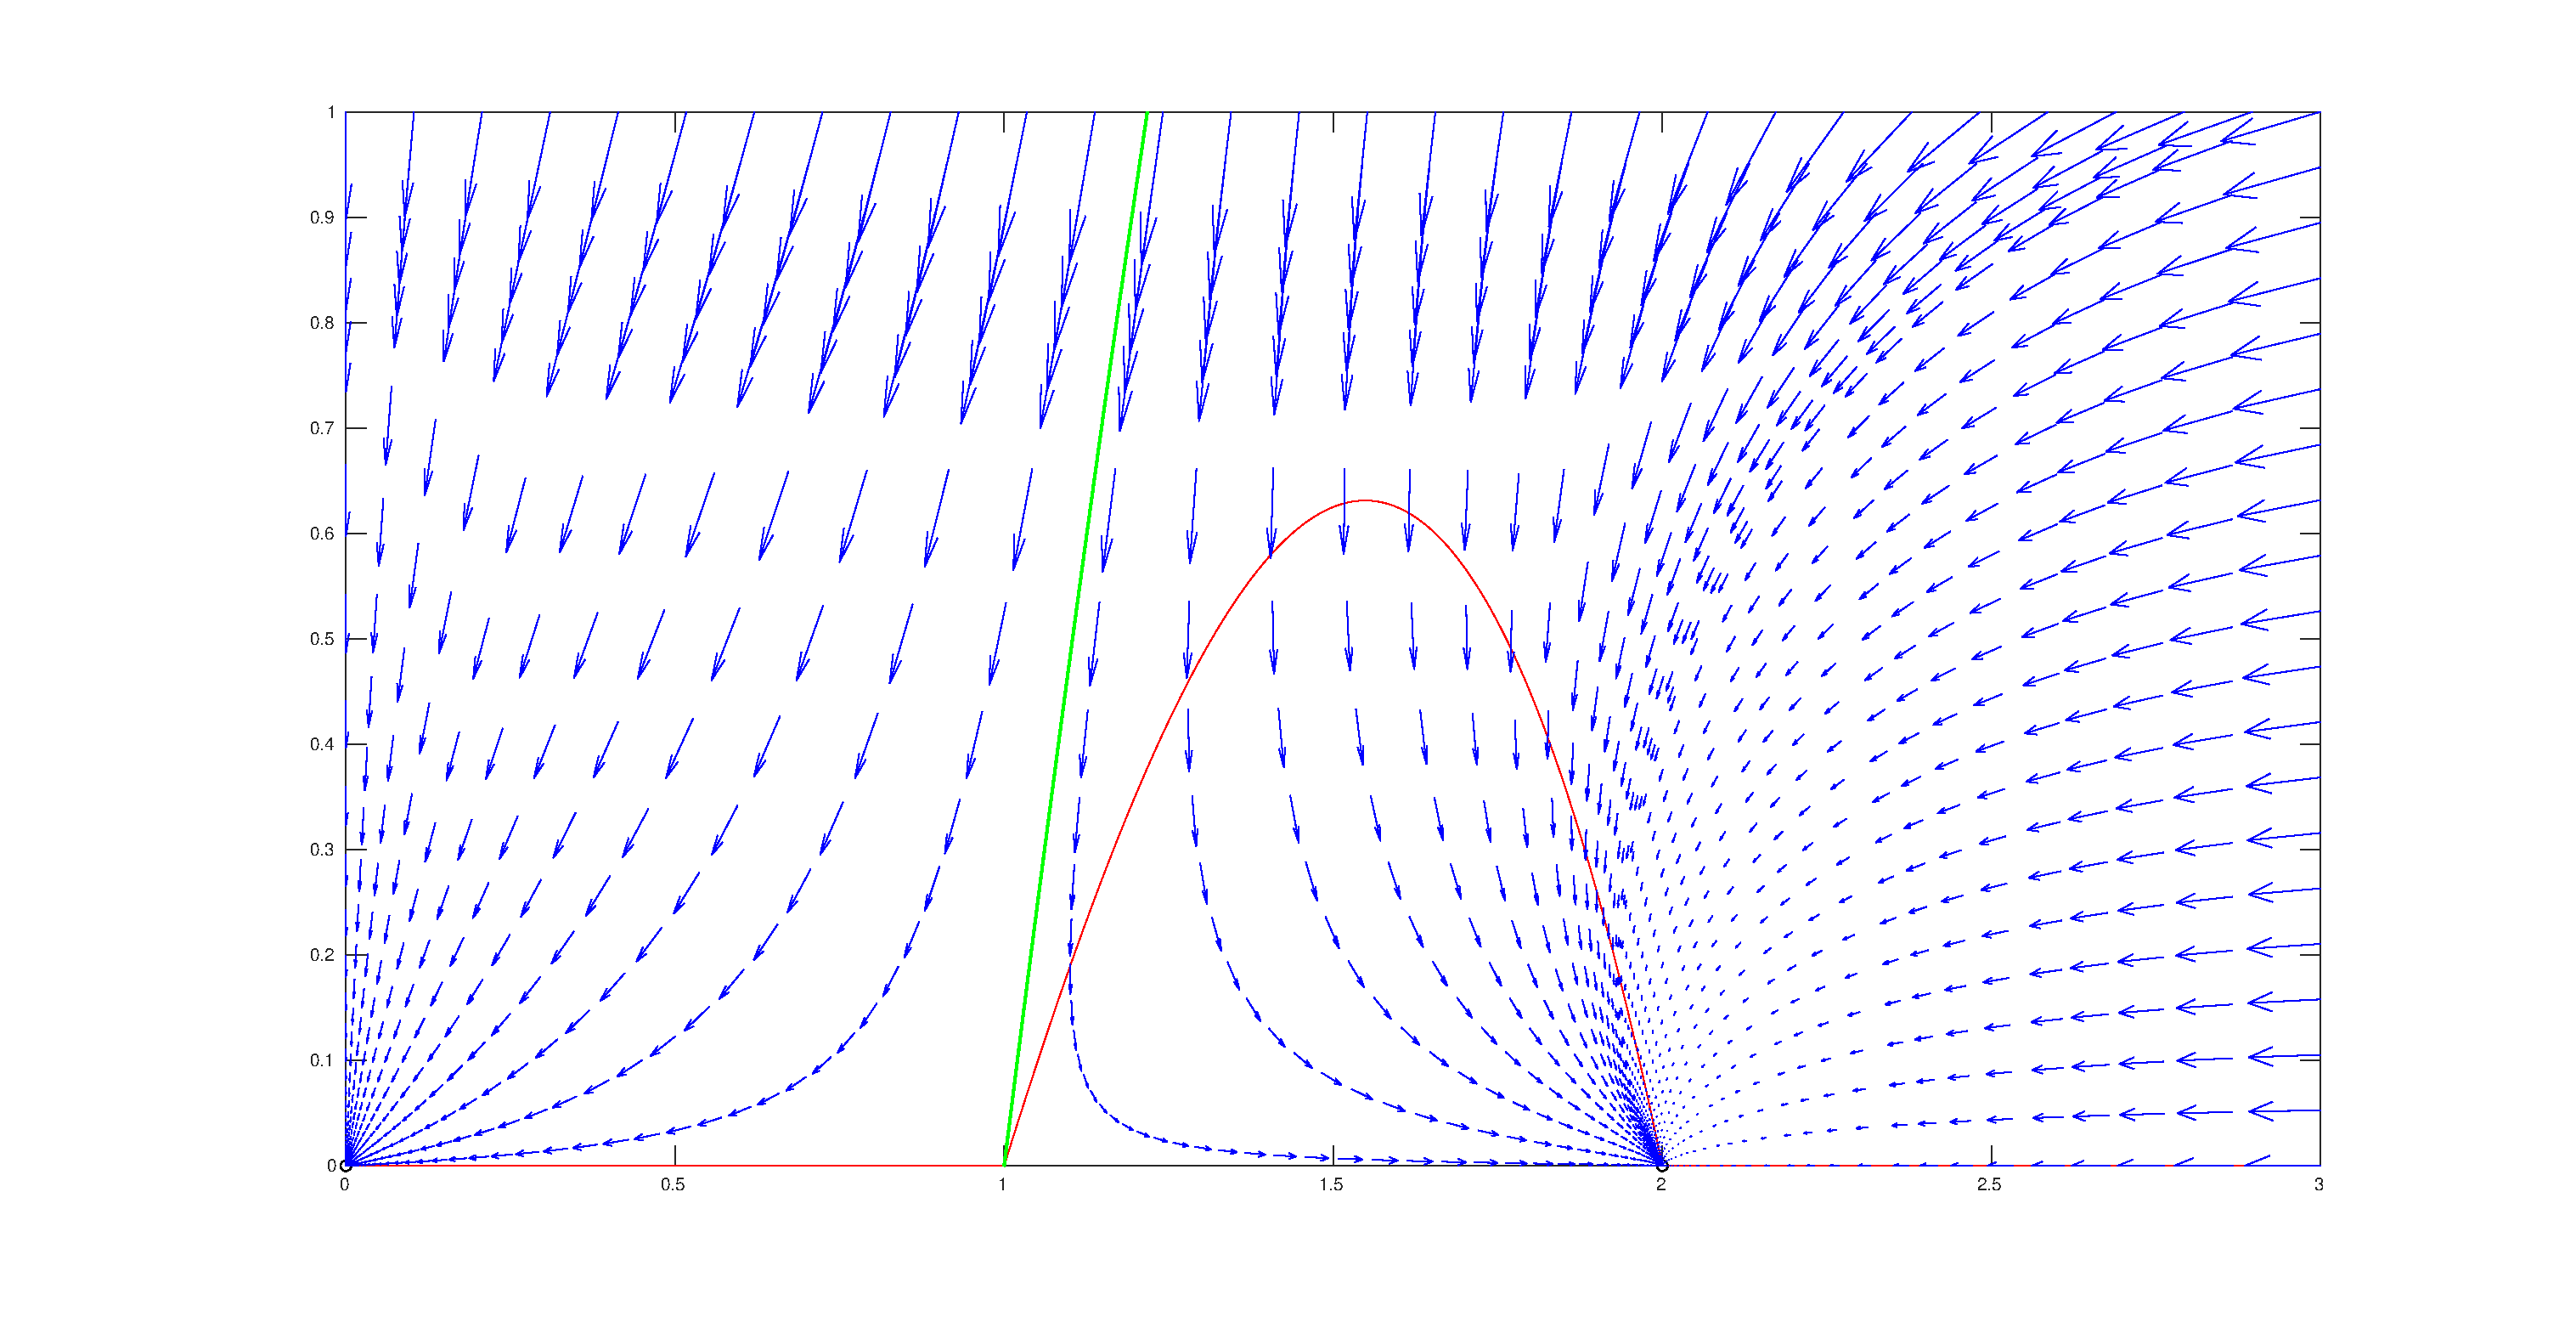
\includegraphics[width=100mm]{ph1.eps}
\caption{Фазовый портрет системы при $a = b = 2$.}
\end{center}
\end{figure}

\paragraph{Область II} Здесь $A_1$ --- репеллер, $A_2$ --- седло, $A_3$ --- устойчивый фокус.
\Pict{phase_2}{Поведение системы в области II}{70}

На границе областей I и II происходит бифуркация, при которой точка $A_2$ разделяется на $A_2$ и $A_3$, в результате 
чего теряет устойчивость. 

Фазовое пространство так же разделяется сепаратрисой седла $A_1$ на две области: зона притяжения $A_0$ и $A_3$.



\begin{figure}[h]
\begin{center}
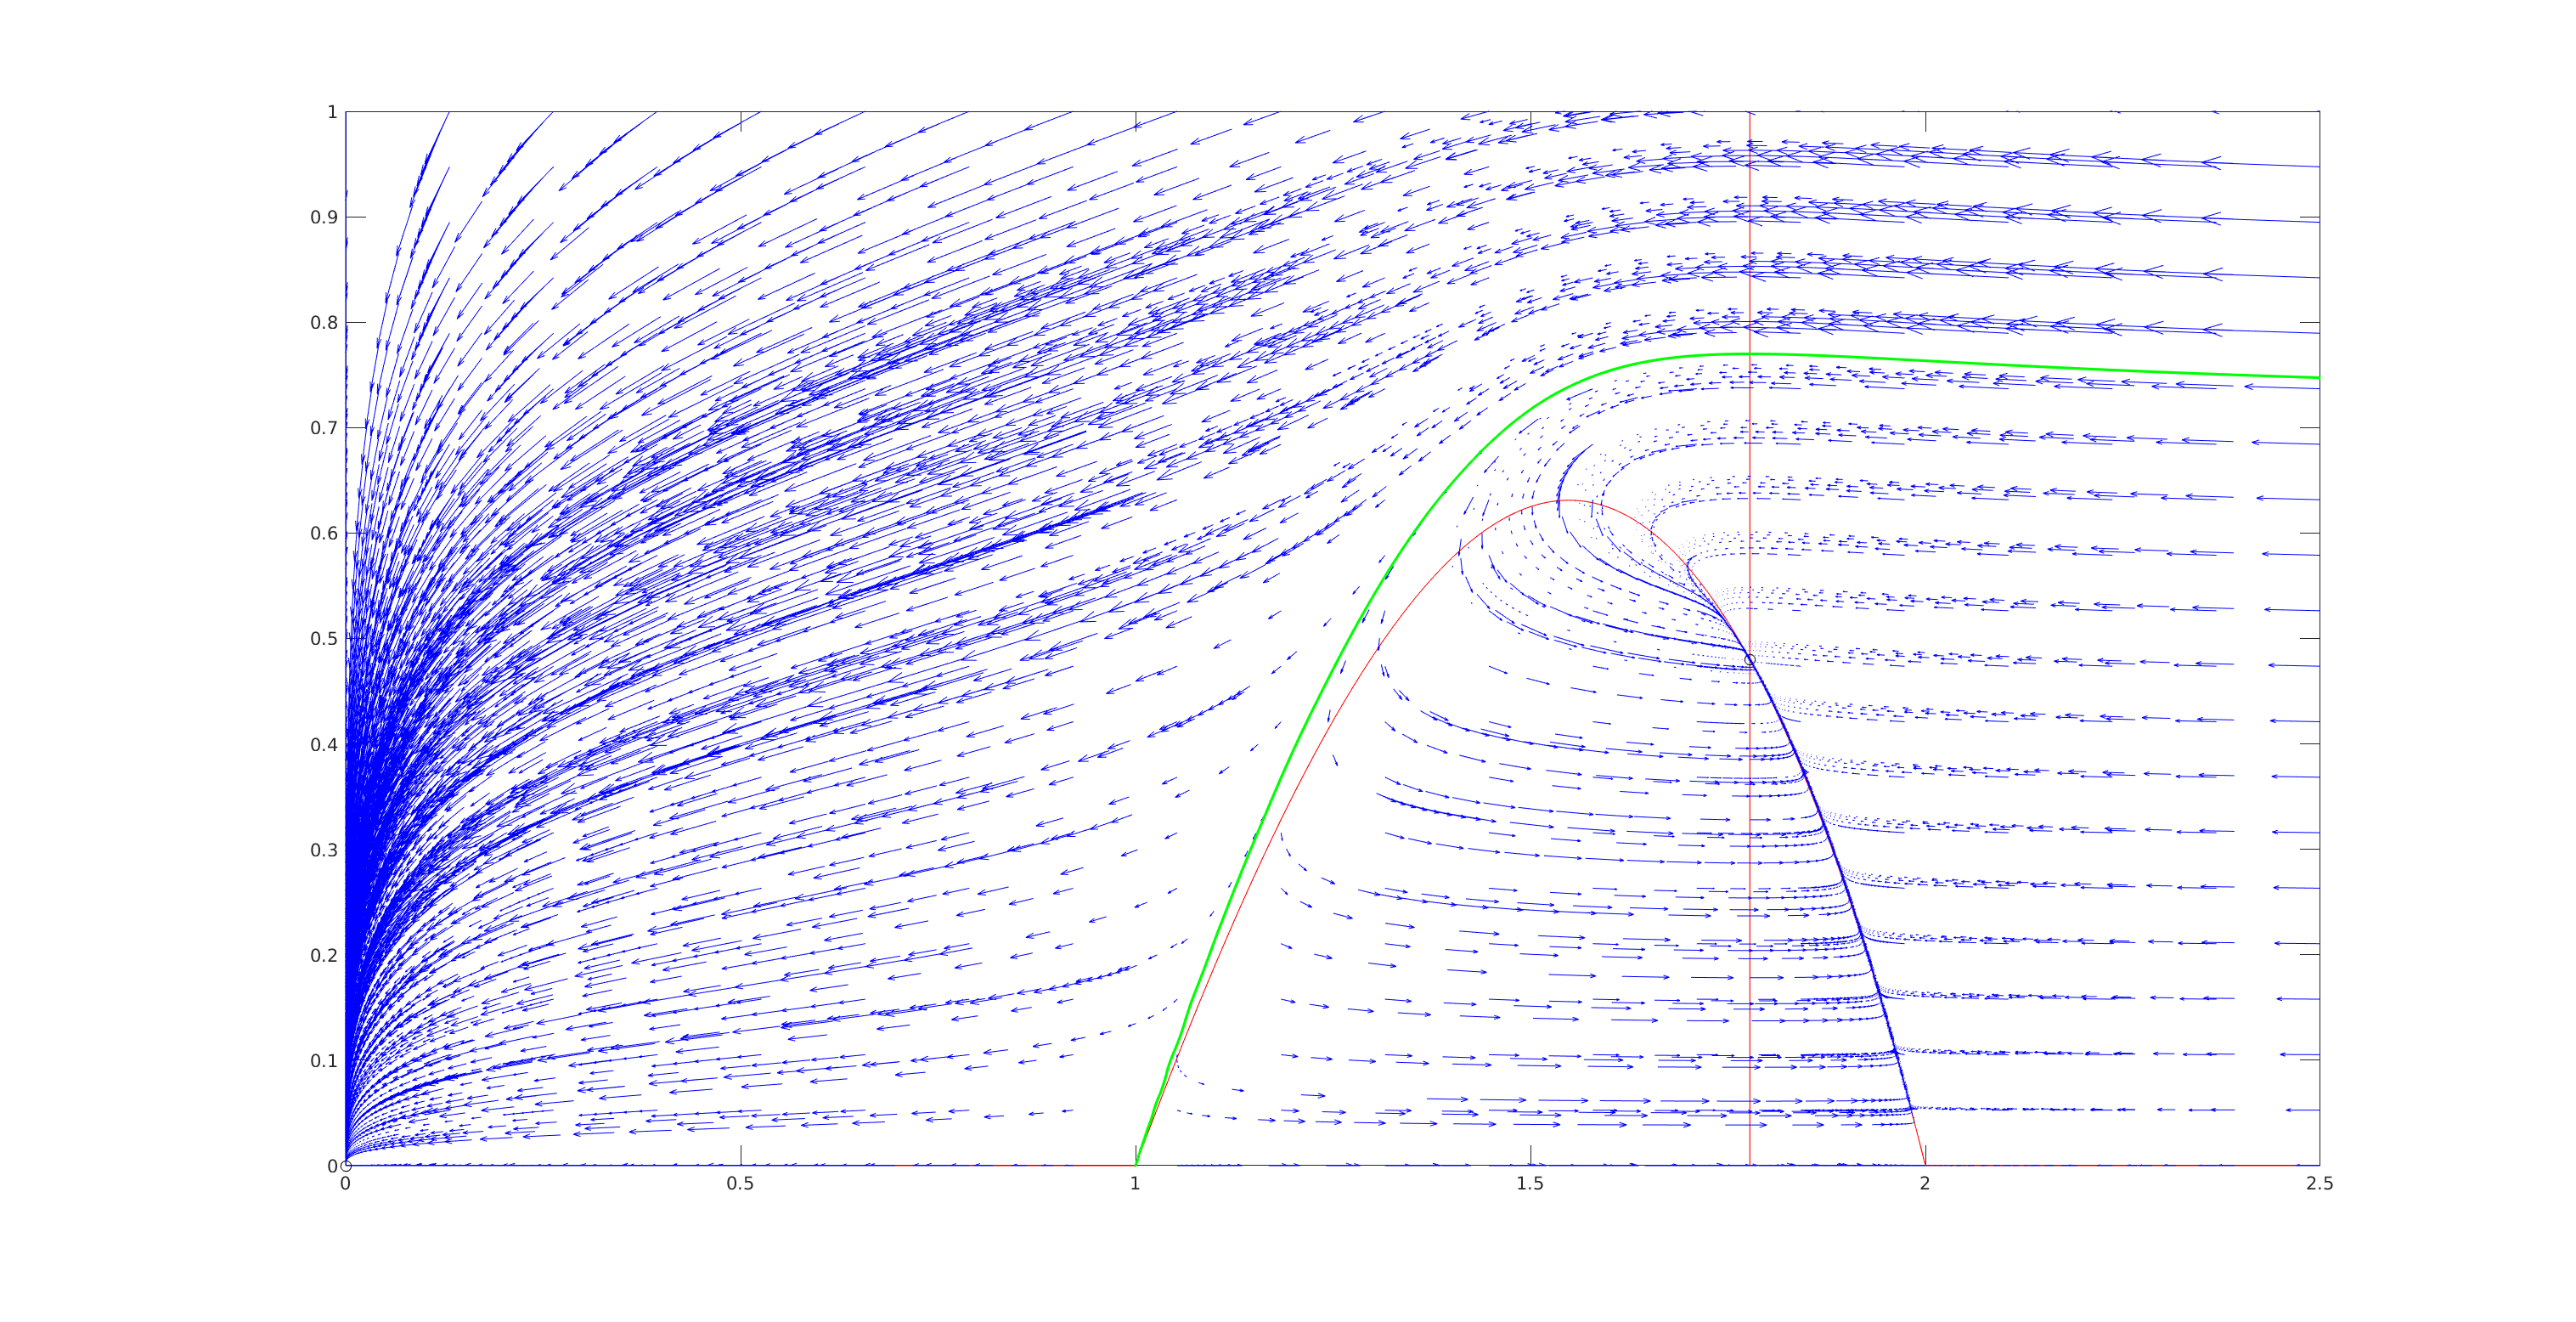
\includegraphics[width=160mm]{ph2.eps}
\caption{Фазовый портрет системы при $a = 2, \ b = 0.64$.}
\end{center}
\end{figure}

\newpage
\paragraph{Область III} $A_1$ --- репеллер, $A_2$  --- седло, $A_3$ --- неустойчивый фокус.
\Pict{phase_3}{Поведение системы в области III}{70}

При переходе из области II в III точка $A_3$ теряет устойчивость, и все траектории стремятся к $A_0$.
Далее будет показано, что при этом в системе возникает бифуркация Пуанкаре-Андронова-Хопфа с мягкой потерей
устойчивости: при значениях параметра, близким к бифуркационным в окрестности неустойчивого фокуса $A_3$ возникает
устойчивый цикл, который затем сливается с сепаратрисой узла $A_2$ и исчезает. Это будет более подробно рассмотрено
в разделе 6.

На фазовом портрете видно, что сепаратриса седла $A_2$ разделяет фазовое пространство на две области, биологическая
интерпретация которых будет дана в разделе 7. 

\begin{figure}[h]
\begin{center}
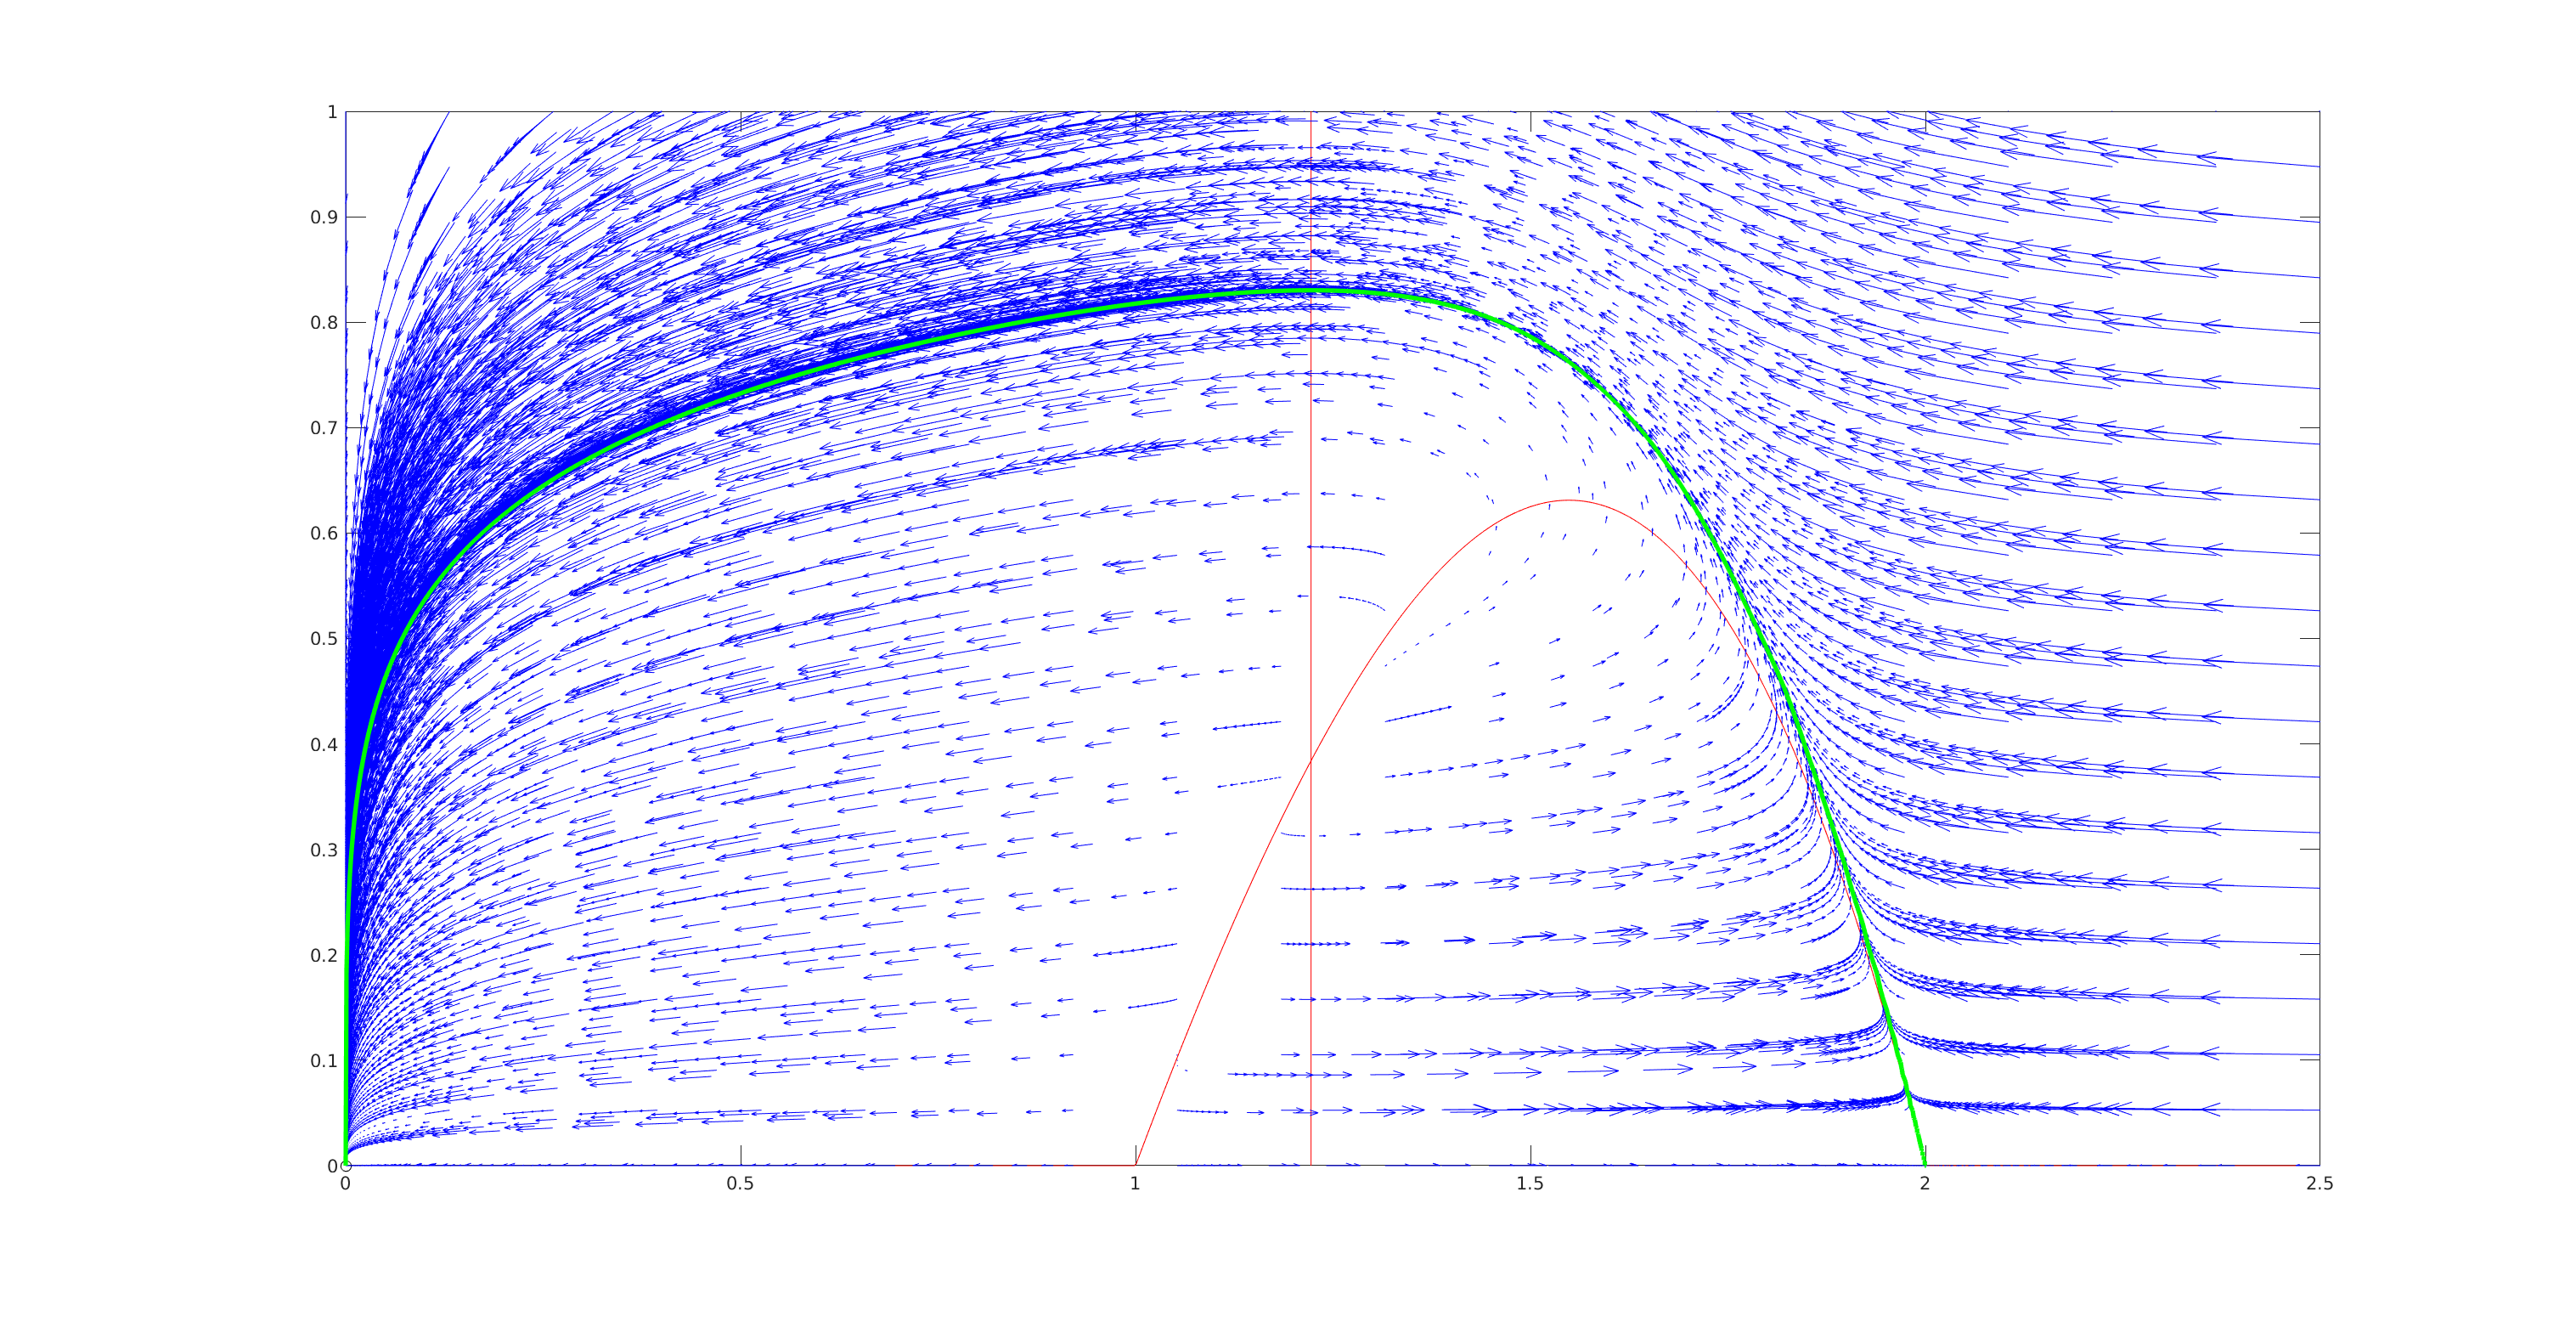
\includegraphics[width=160mm]{ph3.eps}
\caption{Фазовый портрет системы при $a = 2, \ b = 0.55$.}
\end{center}
\end{figure}
\newpage

\newpage
\paragraph{Область VI} $A_1$ --- седло, $A_2$  --- седло.
\Pict{phase_4}{Поведение системы в области IV}{70}

При переходе из области III в IV происходит бифуркация, при которой точки $A_1$ и $A_3$ сливаются, и неподвижная
точка $A_3$ исчезает. Все траектории по-прежнему стремятся к $A_0$.

\begin{figure}[h]
\begin{center}
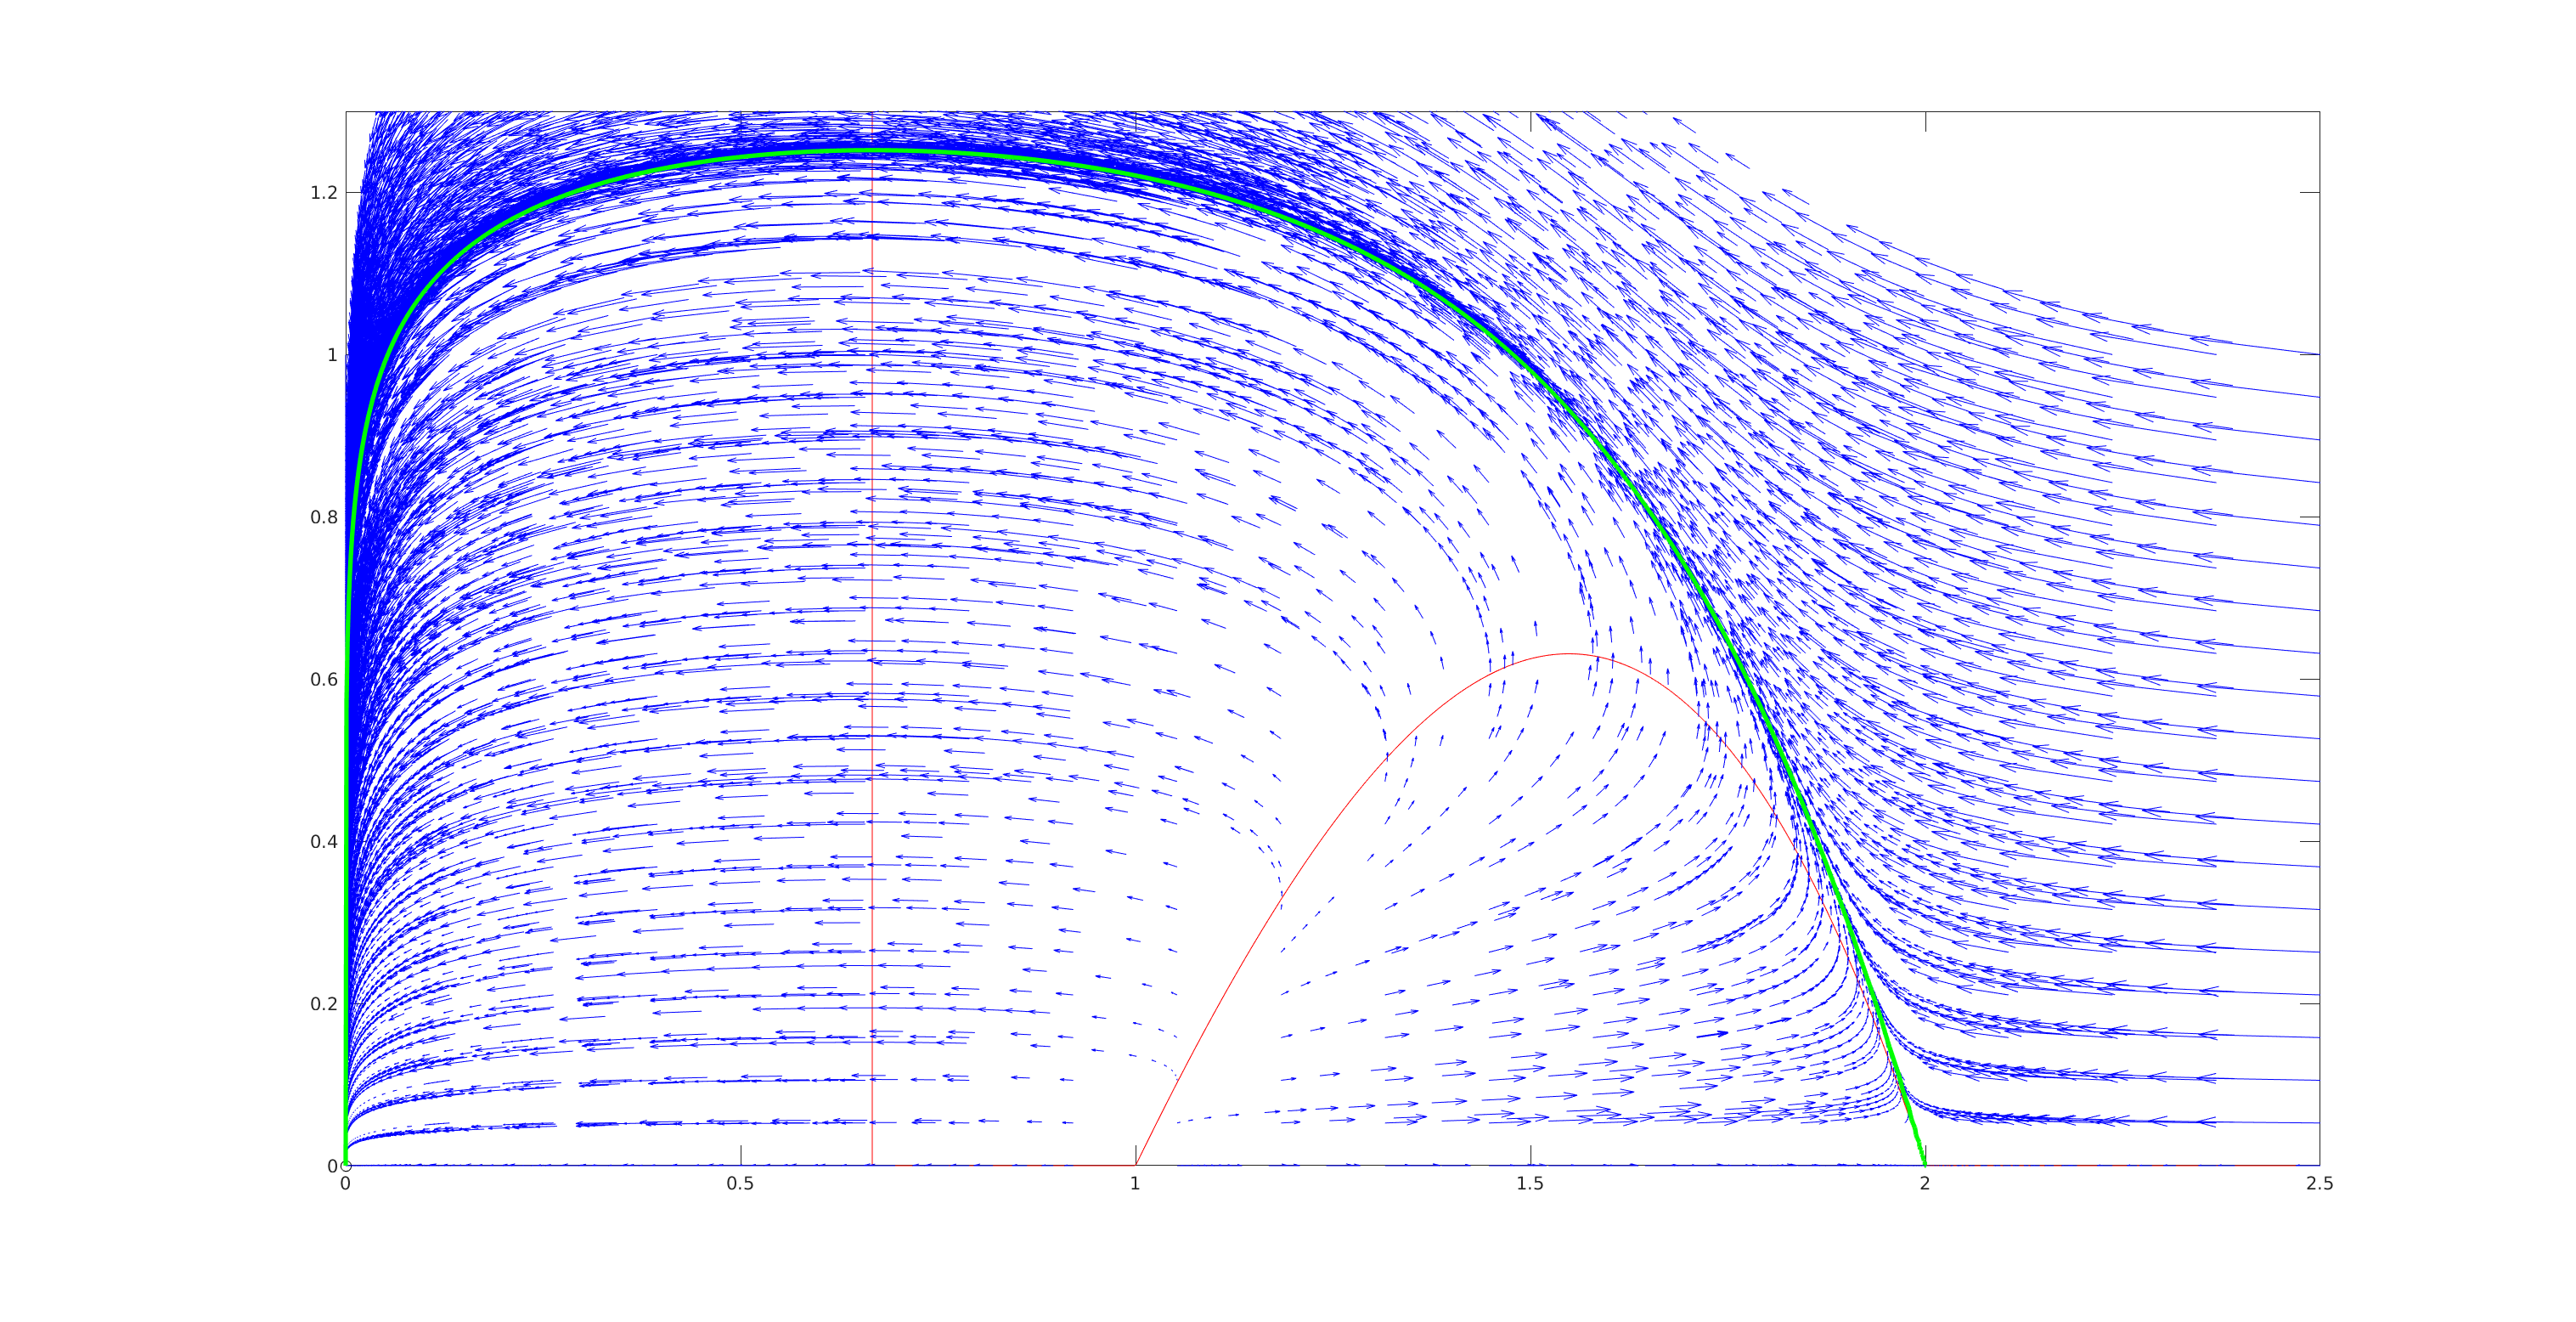
\includegraphics[width=160mm]{ph4.eps}
\caption{Фазовый портрет системы при $a = 2, \ b = 0.4$.}
\end{center}
\end{figure}
\newpage

\section{Бифуркация Пуанкаре-Андронова-Хопфа}
Для проверки бифуркации Пуанкаре-Андронова-Хопфа воспользуемся достаточноым условием, которое можно найти в
\cite{bratus}. В окрестности особой точки функция $f$ представима в виде
$$ f(x) = J(a, b)x + F(x; a, b), \quad F = o(\Norm{x - A_3}).$$

Обозначим $\lambda = \mu + i\omega$ --- собственное значение матрицы $J$. При бифуркационном значении параметров
$a, b$ (на границе областей II и III) $\lambda = i\omega_0$.

Далее, $q$ --- собственный вектор $J$, отвечающий $\lambda$, а $p$ --- собственный вектор $J^T$, отвечающий
$\overline{\lambda}$. Нормализуем их так, чтобы $\Scal{p}{q} = 1$.

Будем теперь, фиксируя $a$, изменять параметр $b$ вблизи бифуркационного значения $b_{cr}$ (полученного из (\ref{restr2})).
С помощью пакета символьных вычислений sympy можно показать, что выполнено условие нетривиальности
$$\left.\dfrac{d\mu(b)}{db}\right|_{b = b_{cr}} \not= 0.$$

Составим теперь комплексную функцию
$$G(z,w) = \Scal{p}{F(zq_1+w\overline{q}_1, zq_2 + w\overline{q}_2)}$$
и вычислим ее частные производные
$$g_{20} = G_{zz}, \quad g_{11} = G_{zw}, \quad g_{21} = G_{zzw}$$
в точке $z = w = 0$.

Тогда первую ляпуновскую величину можно найти по формуле
$$l_1(0) = \dfrac{1}{2\omega_0}\Rea(ig_{20}g_{11} + \omega_0 g_{21}).$$

Ее зависимость от параметра $a$ приведена на графике.

\begin{figure}[h]
\begin{center}
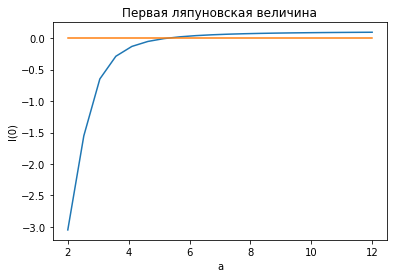
\includegraphics[width=80mm]{lyap.png}
\caption{Зависимость $l_1(0)$ от $a$.}
\end{center}
\end{figure}

Видно, что при $a < 5.2$ (примерно) $l_1(0) < 0$, и происходит субкритическая
бифуркация Пуанкаре-Андронова-Хопфа с мягкой потерей устойчивости, при больших $a$ бифуркация суперкритическая 
с жесткой потерей устойчивости.

\newpage

Проиллюстрируем бифуркацию при $a = 2$.

\begin{figure}[h]
\begin{center}
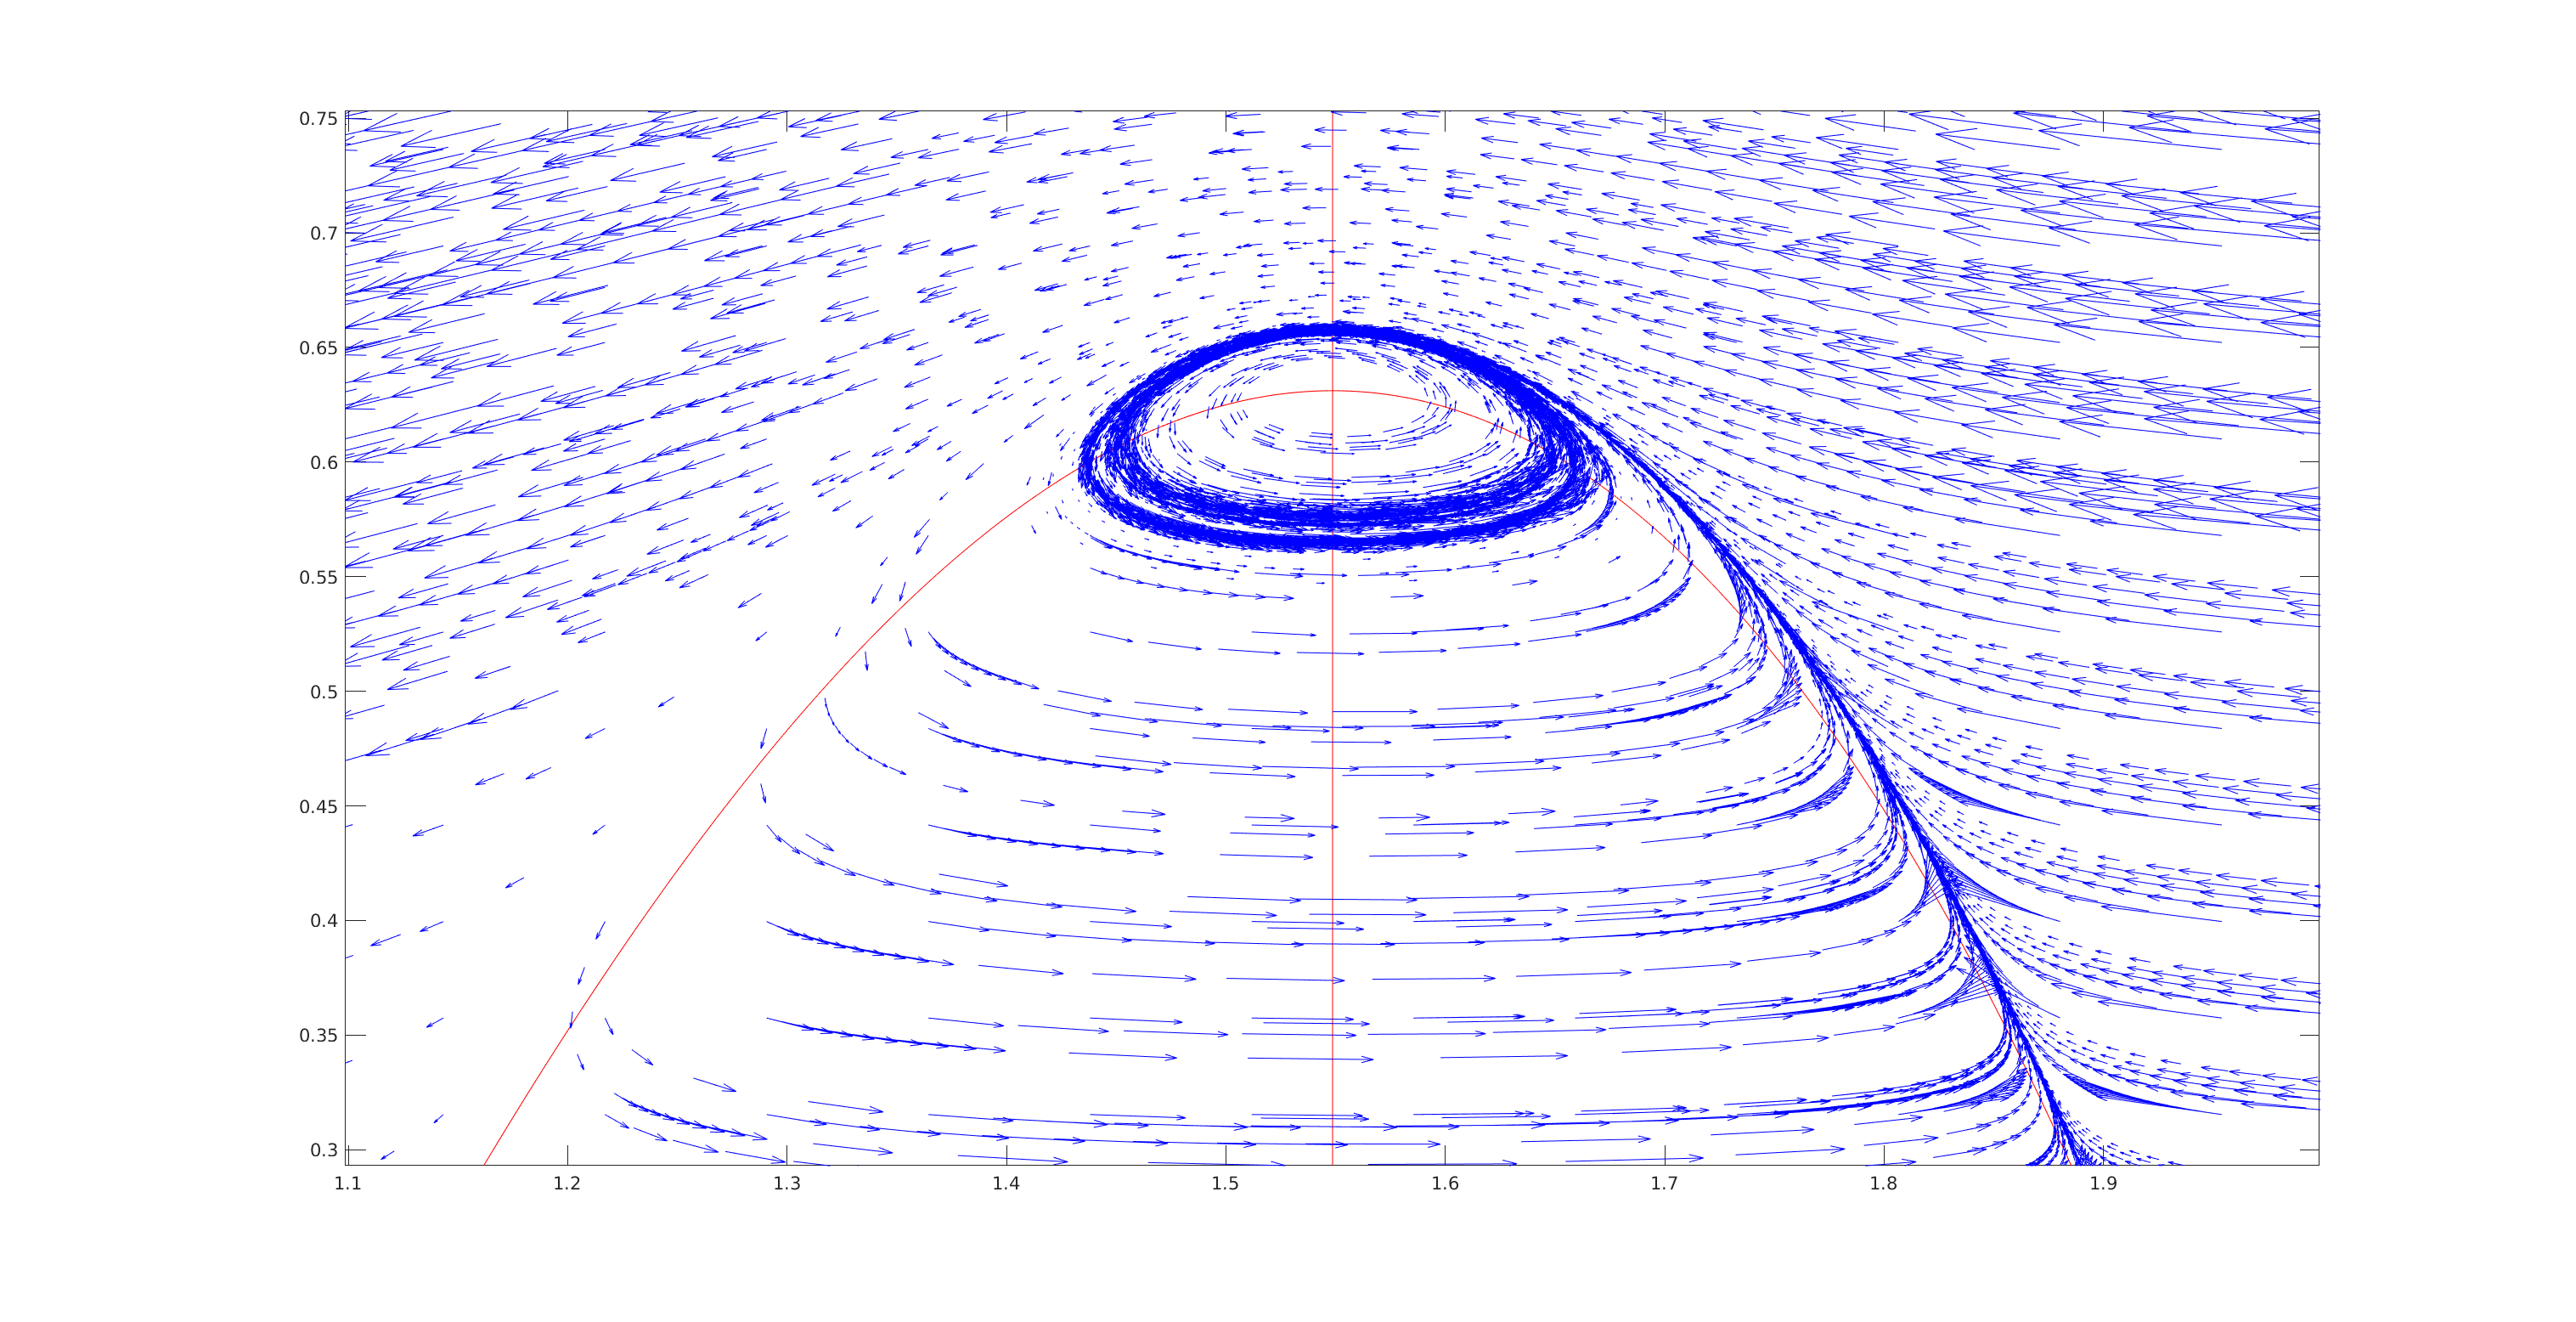
\includegraphics[width=140mm]{bif.eps}
\caption{Бифуркация Пуанкаре-Андронова-Хопфа при $a = 2$.}
\end{center}
\end{figure}

При незначительном уменьшении параметра $b$ вокруг точки $A_3$ появляется устойчивый предельный цикл.

\begin{figure}[h]
\begin{center}
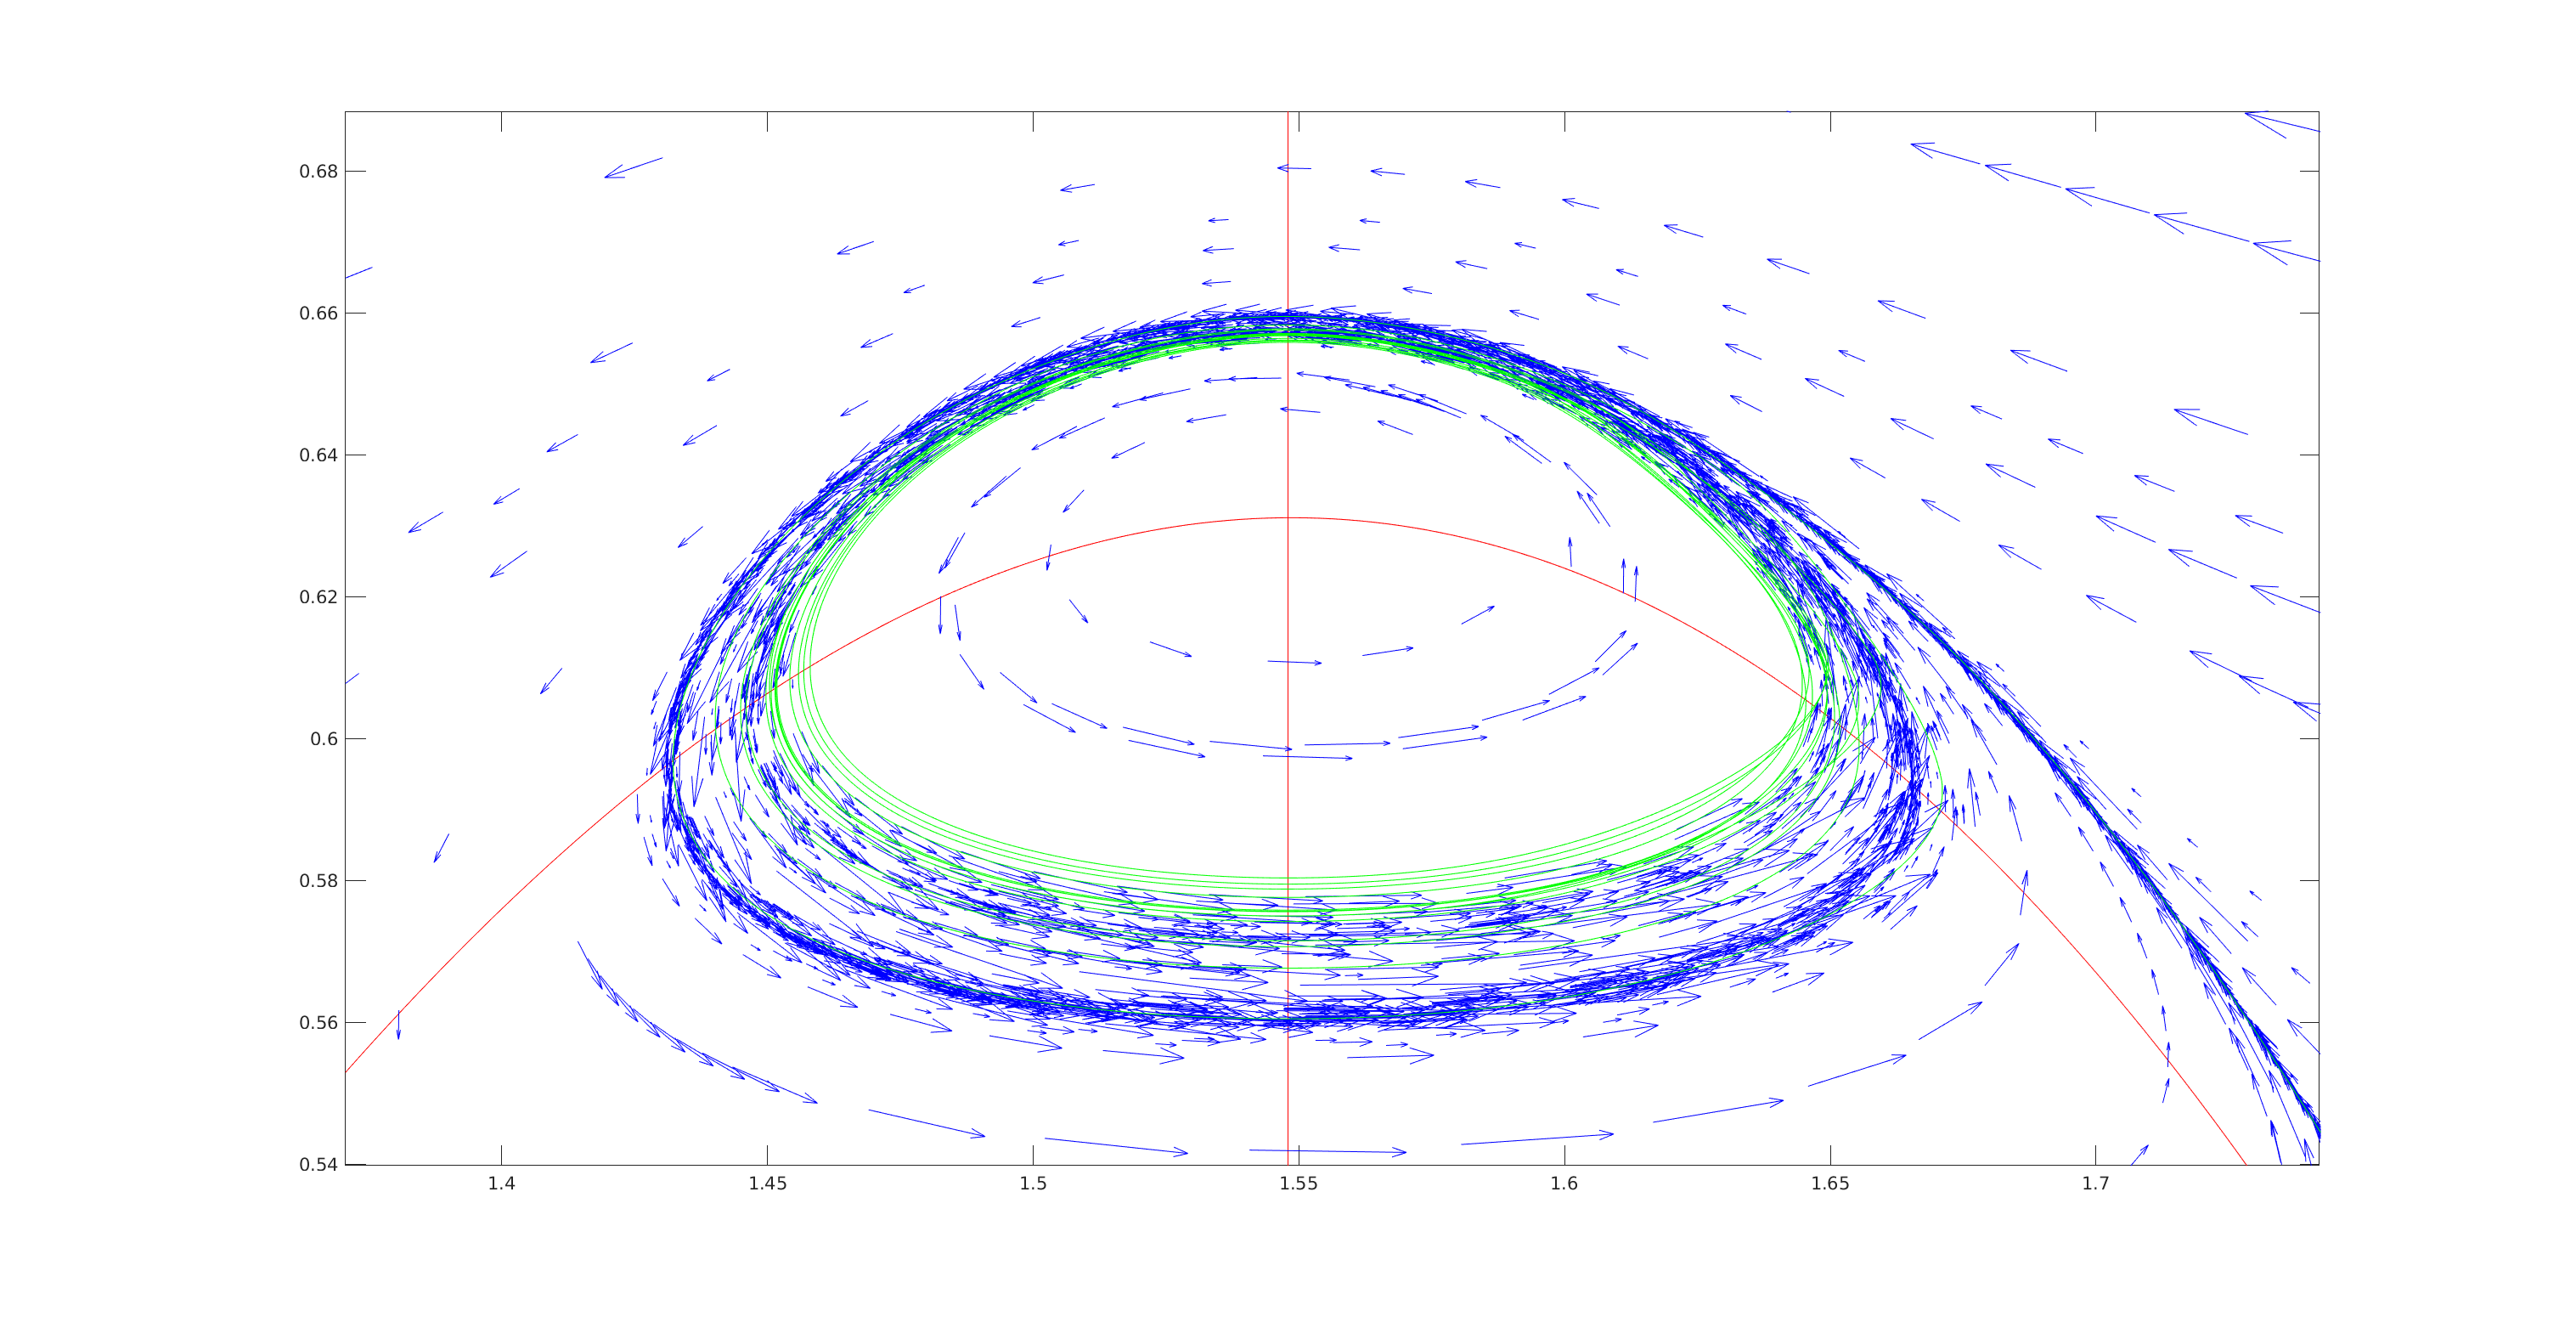
\includegraphics[width=140mm]{cycle.eps}
\caption{Предельный цикл при $a = 2$.}
\end{center}
\end{figure}

При дальнейгем уменьшении параметра $b$ цикл сливается с сепаратрисой седла $A_2$ и исчезает. Это 
согласуется с теорией, так как результат
теоремы о бифуркации Пуанкаре-Андронова-Хопфа описывает топологическую структуру фазового портрета лишь в
некоторой окрестности особой точки.

\newpage

\begin{figure}[h]
\begin{center}
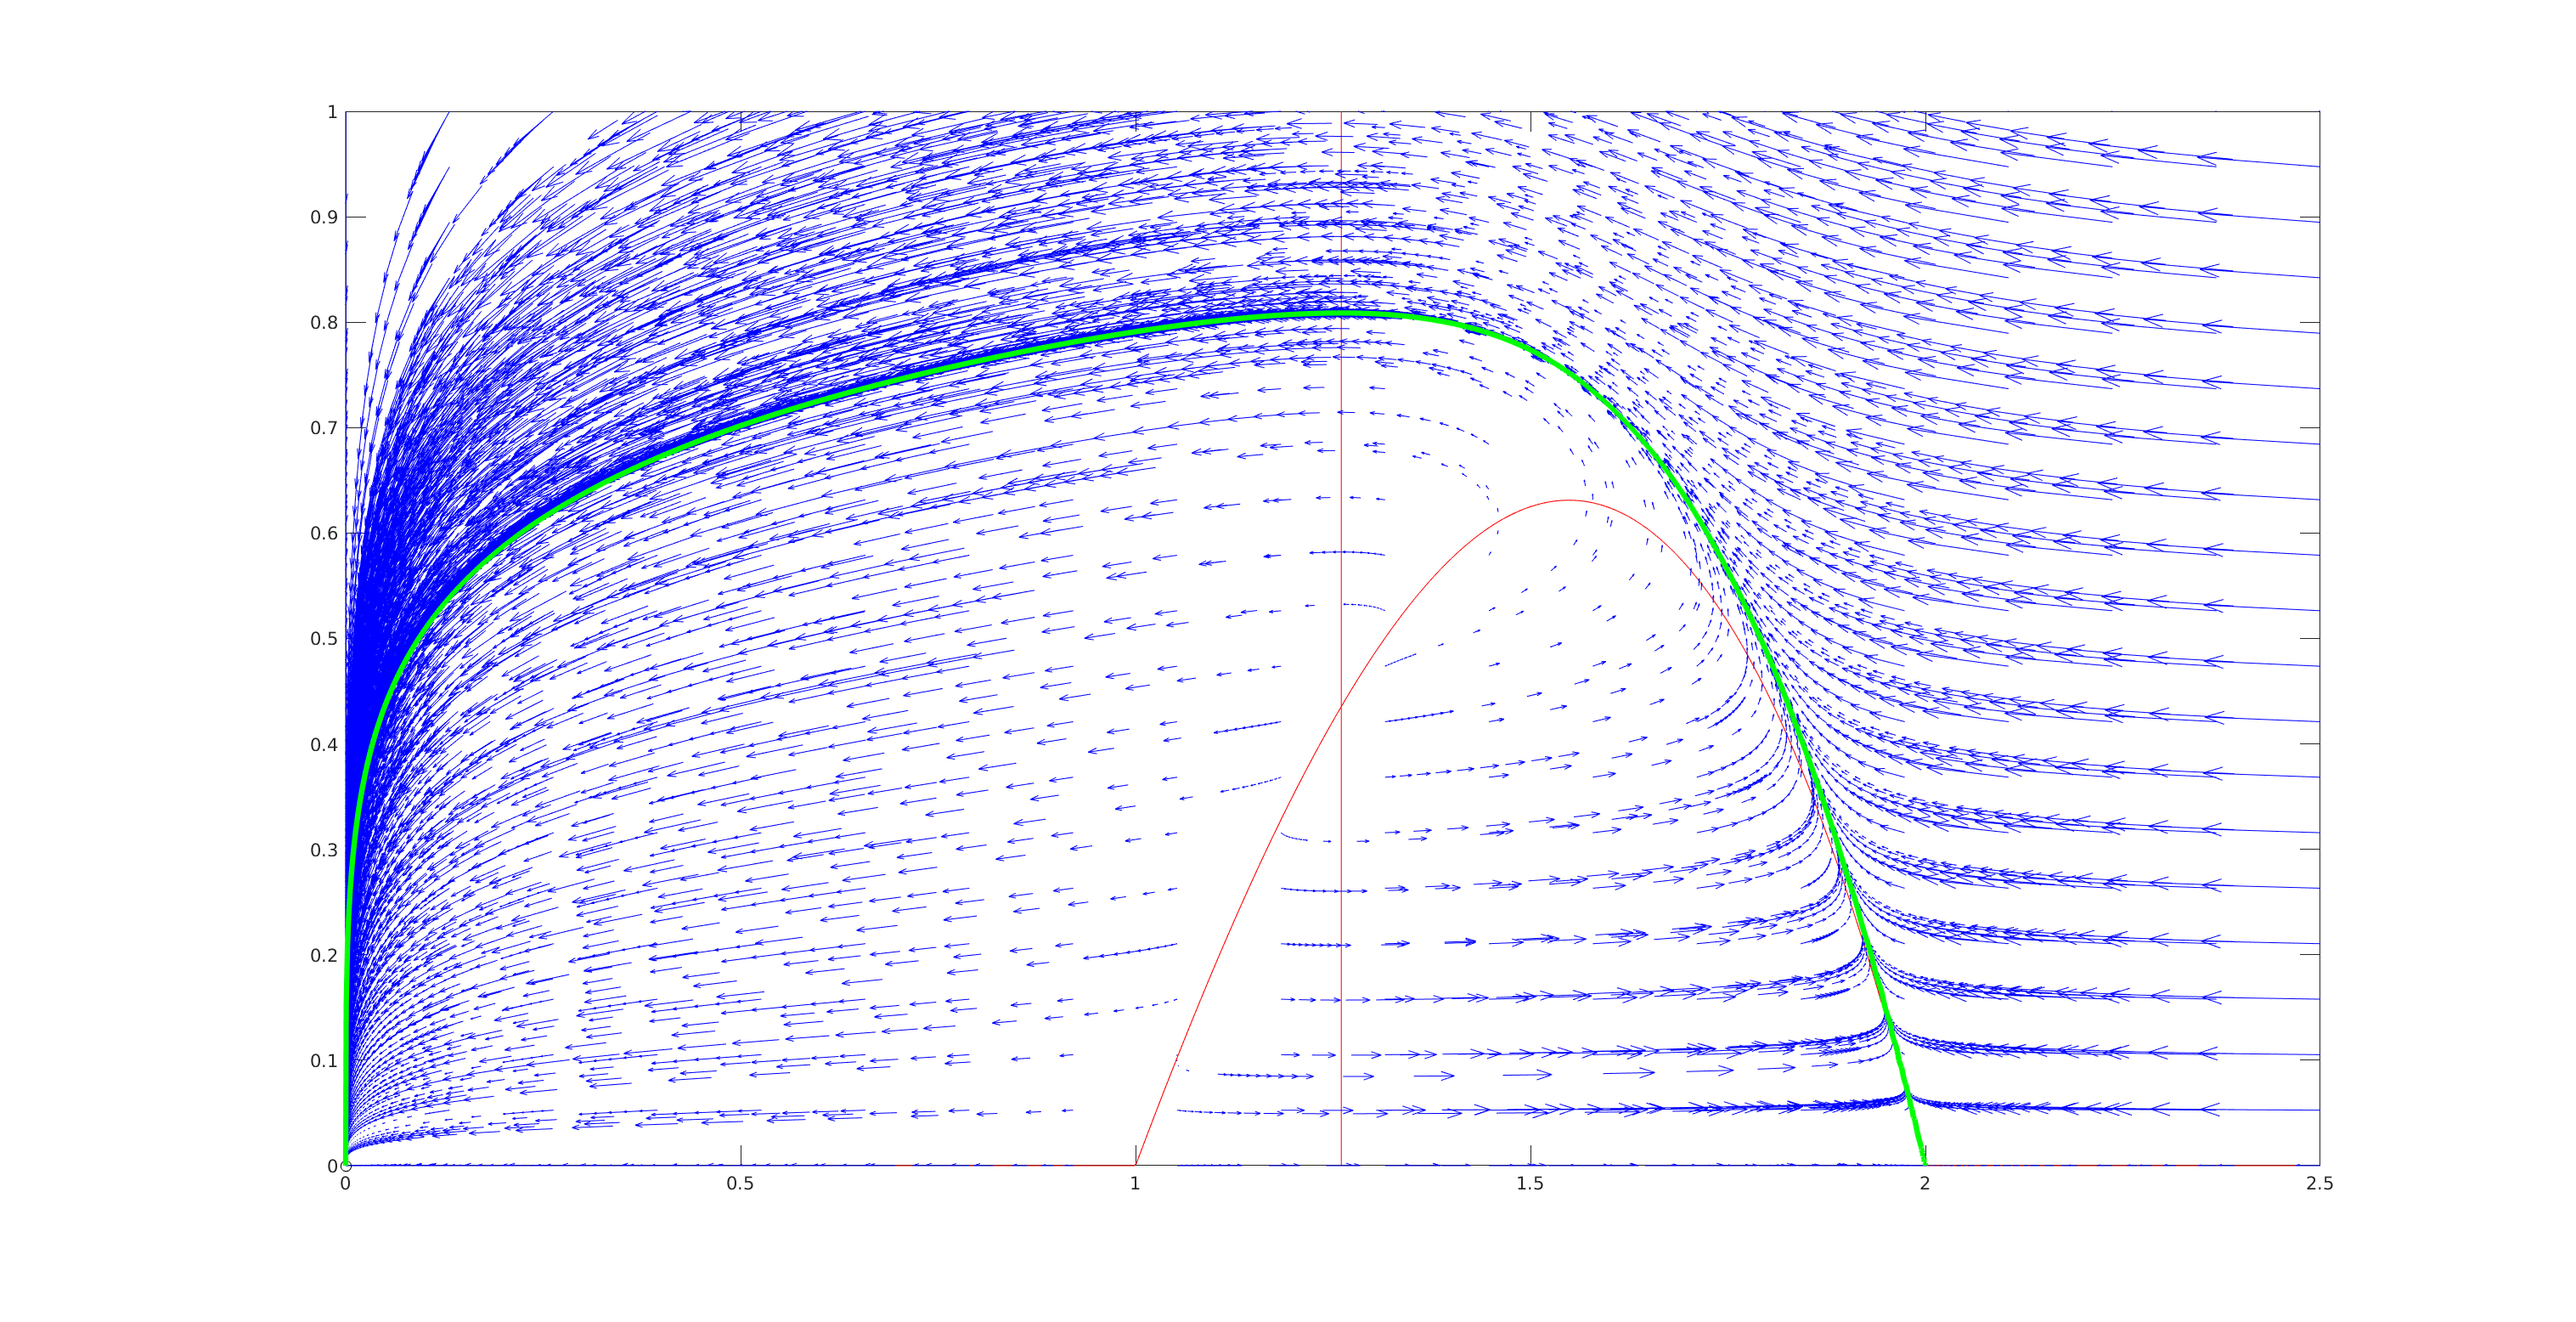
\includegraphics[width=140mm]{sep.eps}
\caption{Загадочное исчезновение цикла.}
\end{center}
\end{figure}

\section{Биологическая интерпретация результатов}

\paragraph{Область I} Из-за высокой смертности хищников их популяция вымирает независимо от числа жертв:
ограниченность трофической функции хищника приводит к тому, что энергии, полученной хищником при взаимодействии с популяцией жертв,
не хватает для поддержания численности собственной популяции. Популяция жертв либо вымирает, либо стабилизируется
в положении устойчивого равновесия. Сепаратриса отделяет
зону, в которой численности жертв достаточно для избежания вымирания.

\paragraph{Область II} В этом и только в этом случае существует устойчивое положение равновесия, допускающее сосуществование 
популяций. Однако при значительном уменьшении числа жертв, обе популяции вымирают, как и в случае сильного
увеличения числа хищников, которое также влечет за собой сокращение популяции жертв и вымирание. 

\paragraph{Область III} Здесь также существует нетривиальное равновесие, при котором численность обеих популяций
положительна, однако сколь угодно малое отклонение от него приводит к росту числа хищников, затем сокращению
числа жертв и полному вымиранию обеих популяций. При этом возможны три сценария:
\begin{enumerate}
\item Большое число жертв в начальный момент приводит к быстрому росту численности хищников, число жертв же
убывает из-за внутривидовой конкуренции и разросшейся популяции хищников, попадая в критическую зону $u < 1$.
\item Начальное условие находится под $u$-нуль-изоклиной. Тогда из-за благоприятных условий численность
жертв растет, приводя к росту числа хищников и повторению прошлого сценария.
\item Изначальное число жертв мало, и из-за большого числа хищников уменьшается до критического значения, что
также приводит к вымиранию.
\end{enumerate}

\paragraph{Область IV} Как и в прошлом случае, обе популяции вымирают. В обоих случаях это связано со слишком
низкой смертностью хищников: их популяция разрастается, число жертв уменьшается до критического уровня, 
при котором восстановление невозможно. Сценарии вымирания абслютно аналогичны сценариям в области III.

\newpage
\begin{thebibliography}{0}
\bibitem{bratus}
	Братусь~А.С., Новожилов~А.С., Платонов~А.П. Динамические системы и модели биологии. М.: ФИЗМАТЛИТ, 2010. 
\end{thebibliography}


\end{document}